\chapter{Introduction to droplet impact dynamics}

\section{Contact angle}
When a gas-liquid interface meets a solid surface, at the point of contact of three phases the liquid makes an angle with the surface. This measures the wettability of 
the solid surface for that liquid. The contact angle is given by Youngs equation, which is sum of all the surface forces at that point ( See Figure \ref{Fig:Contact_angle} ).
\begin{wrapfigure}{r}{0.5\textwidth}
  \begin{center}
    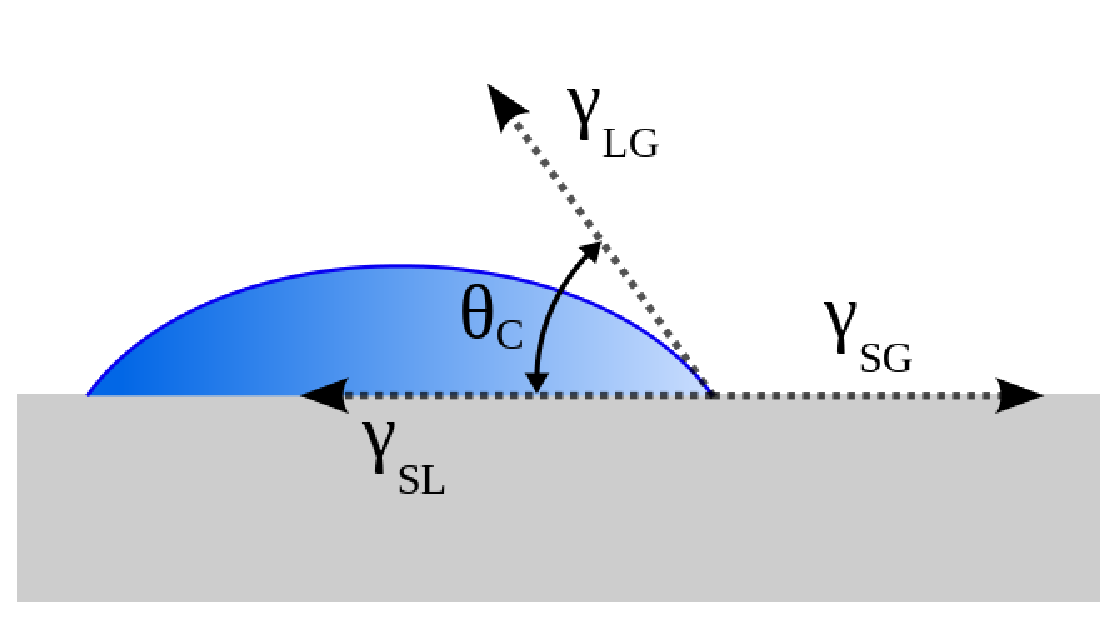
\includegraphics[width=0.48\textwidth]{Contact_angle.eps}
  \end{center}
  \caption{Contact angle}
  \label{Fig:Contact_angle}
\end{wrapfigure}
\begin{equation}
 \boxed{ \begin{align}
 &\gamma_{SG} -\gamma_{SL} - \gamma_{LG} \cos \theta =0  \\
 &\cos \theta =\frac{\gamma_{SG} -\gamma_{SL}}{\gamma_{LG}} 
 \end{align}
 }
\end{equation}
\begin{figure}
 \centering
 \subfloat[t = 26.2 ]{%
      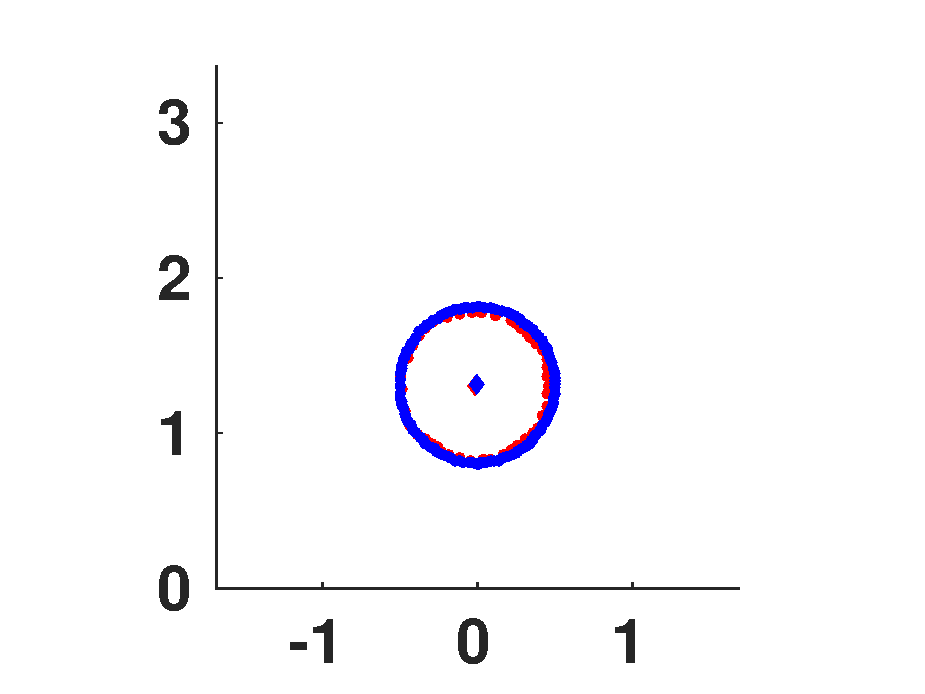
\includegraphics[width=0.3\textwidth]{clanet-1.eps}
      }
  \subfloat[t = 27.1 ]{%
      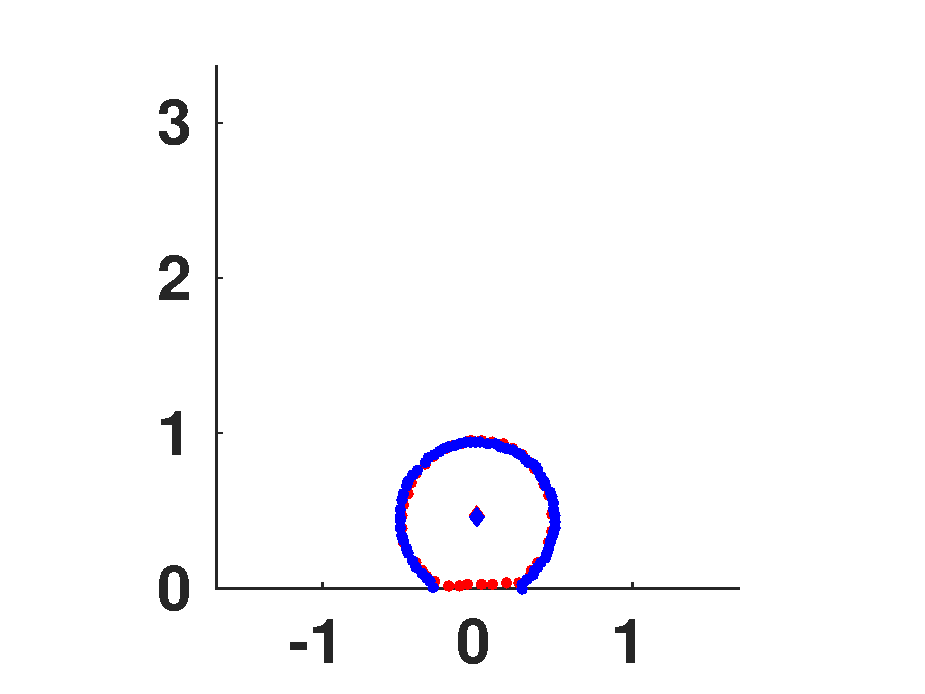
\includegraphics[width=0.3\textwidth]{clanet-2.eps}
      } 
       \subfloat[t = 28.0 ]{%
      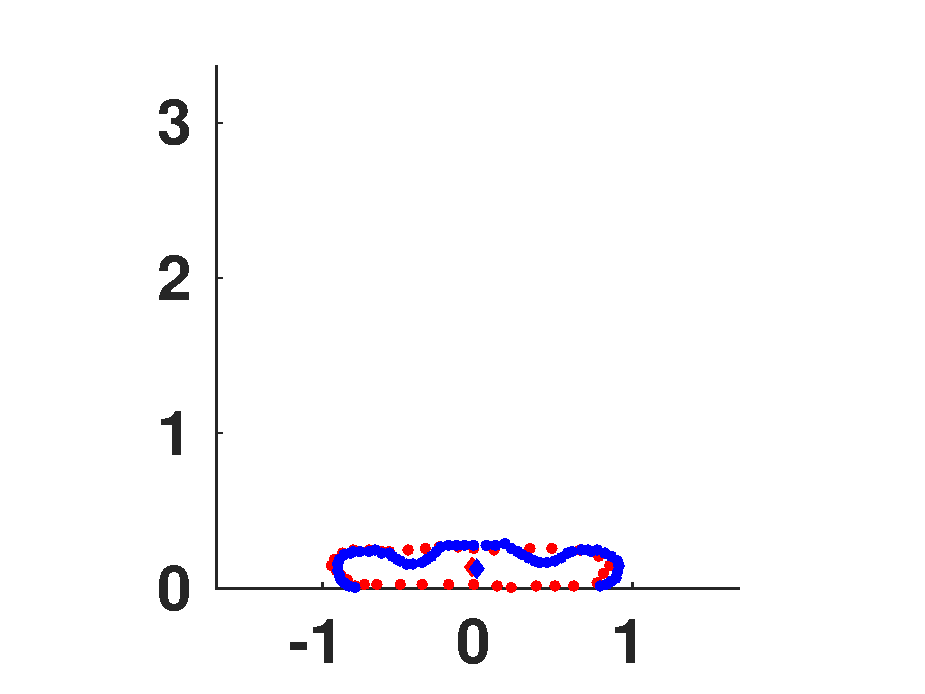
\includegraphics[width=0.3\textwidth]{clanet-3.eps}
      }\\
       \subfloat[t = 28.9 ]{%
      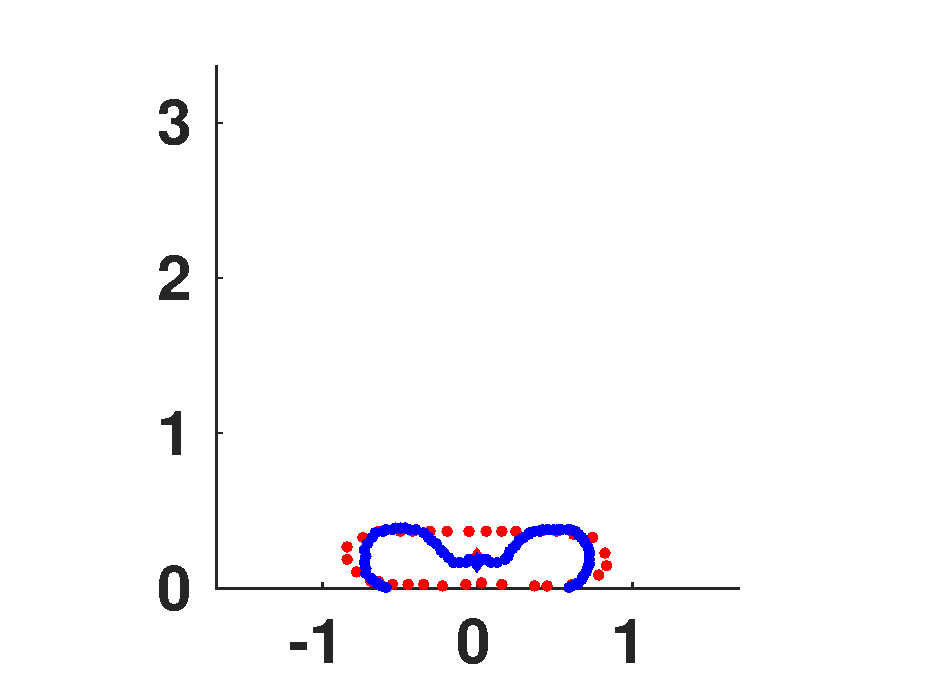
\includegraphics[width=0.3\textwidth]{clanet-4.eps}
      }
    \subfloat[t = 29.8 ]{%
      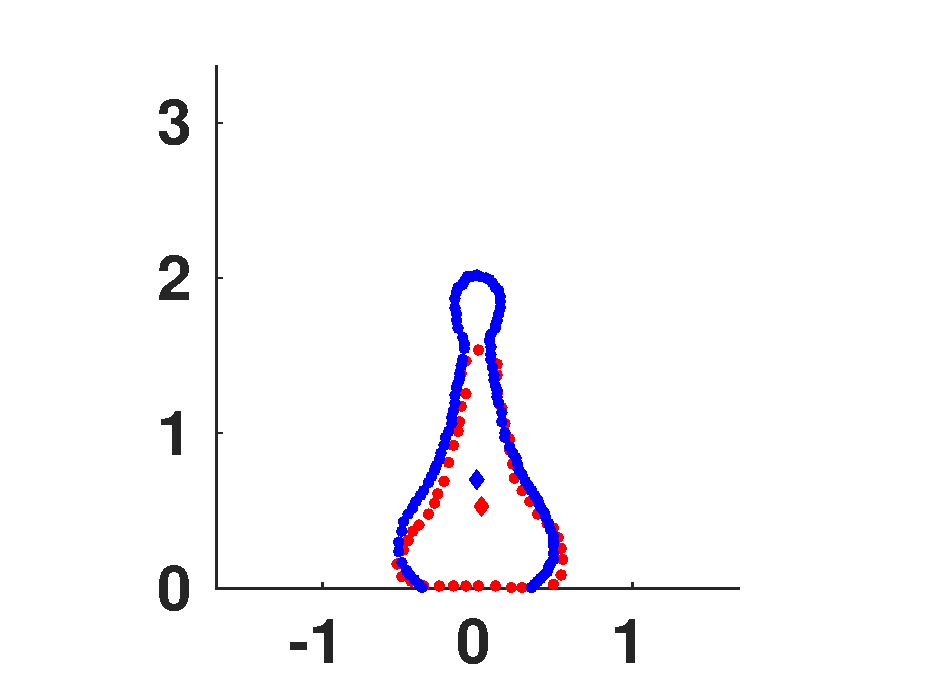
\includegraphics[width=0.3\textwidth]{clanet-5.eps}
      }
       \subfloat[t = 30.7 ]{%
      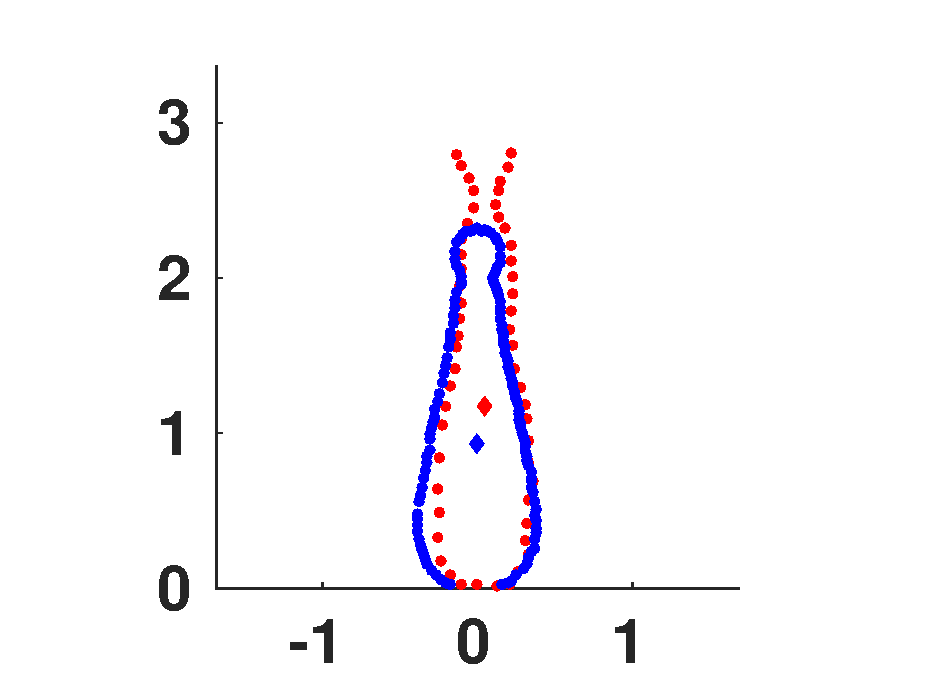
\includegraphics[width=0.3\textwidth]{clanet-6.eps}
      }\\
       \subfloat[t = 31.6 ]{%
      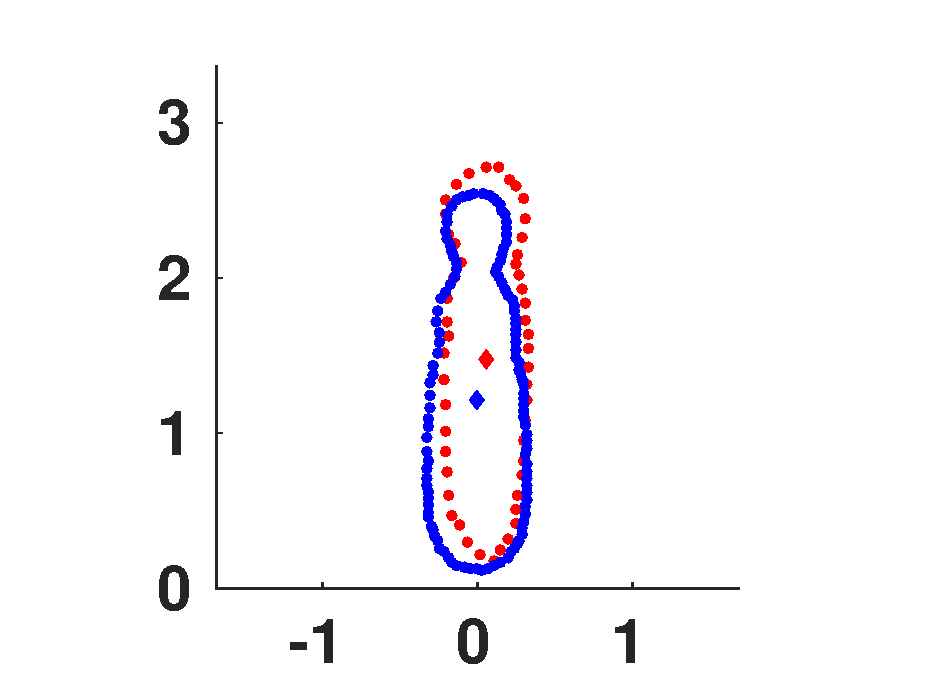
\includegraphics[width=0.3\textwidth]{clanet-7.eps}
      }
       \subfloat[t = 32.5 ]{%
      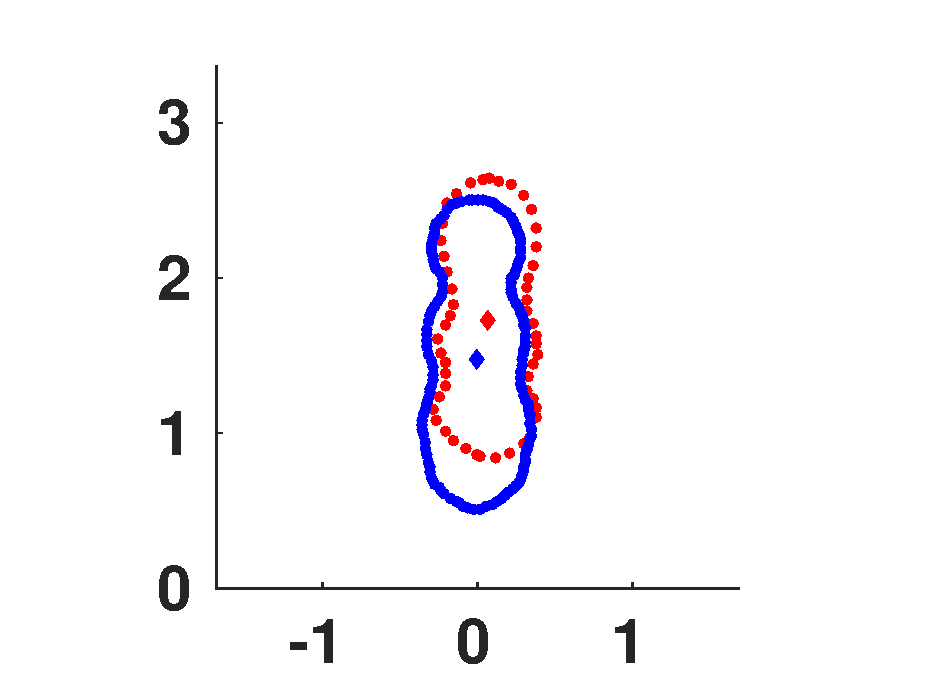
\includegraphics[width=0.3\textwidth]{clanet-8.eps}
      }
       \subfloat[t = 33.4 ]{%
      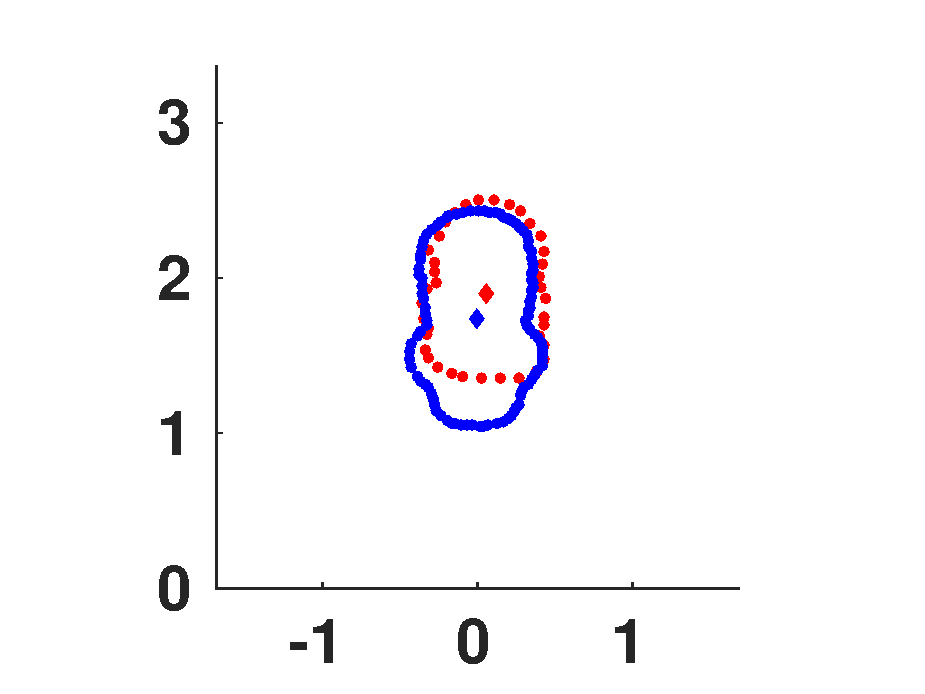
\includegraphics[width=0.3\textwidth]{clanet-9.eps}
      }
 \caption{Interface Gerris simulation data(BLUE) with \cite{Clanet2004} experimental data(RED)}
 \label{Fig:gs6}
 \end{figure}
 \begin{figure}
 \centering
 \subfloat[t = 15.6 ]{%
      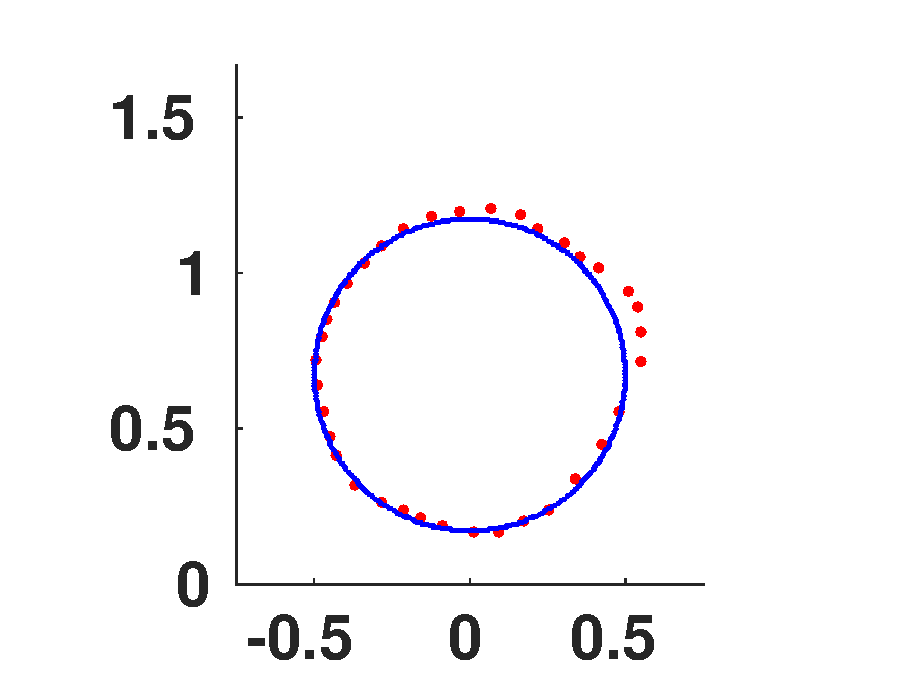
\includegraphics[width=0.3\textwidth]{wang-1.eps}
      }
  \subfloat[t = 16.0 ]{%
      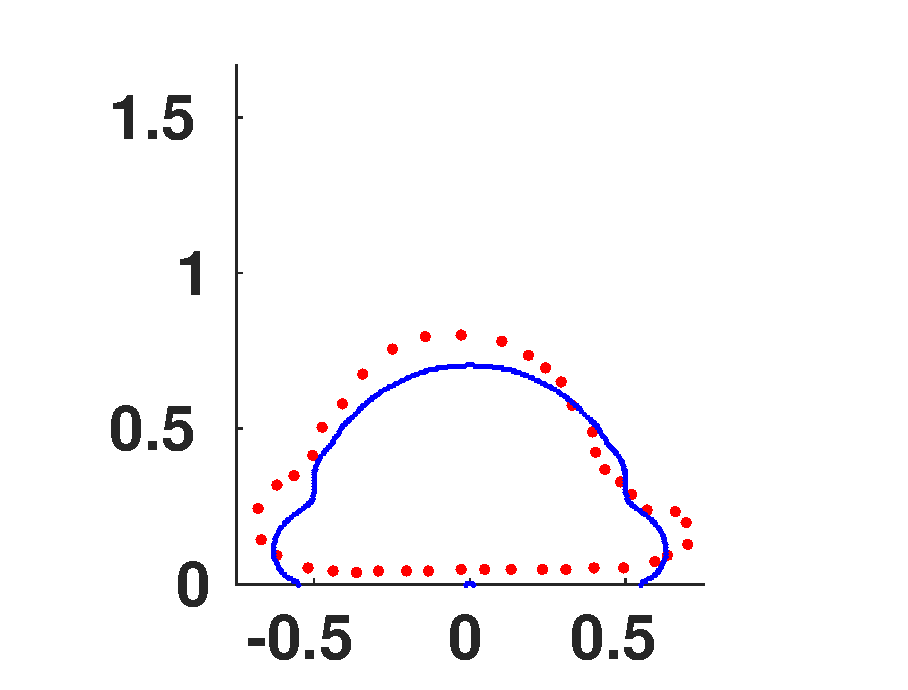
\includegraphics[width=0.3\textwidth]{wang-2.eps}
      } 
       \subfloat[t = 17.0 ]{%
      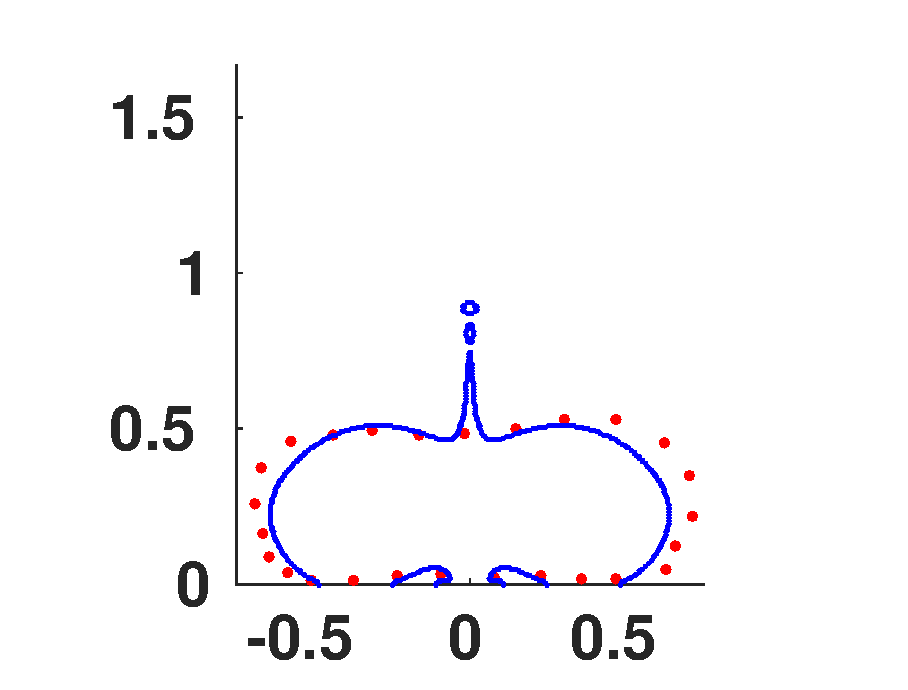
\includegraphics[width=0.3\textwidth]{wang-3.eps}
      }\\
       \subfloat[t = 18.1 ]{%
      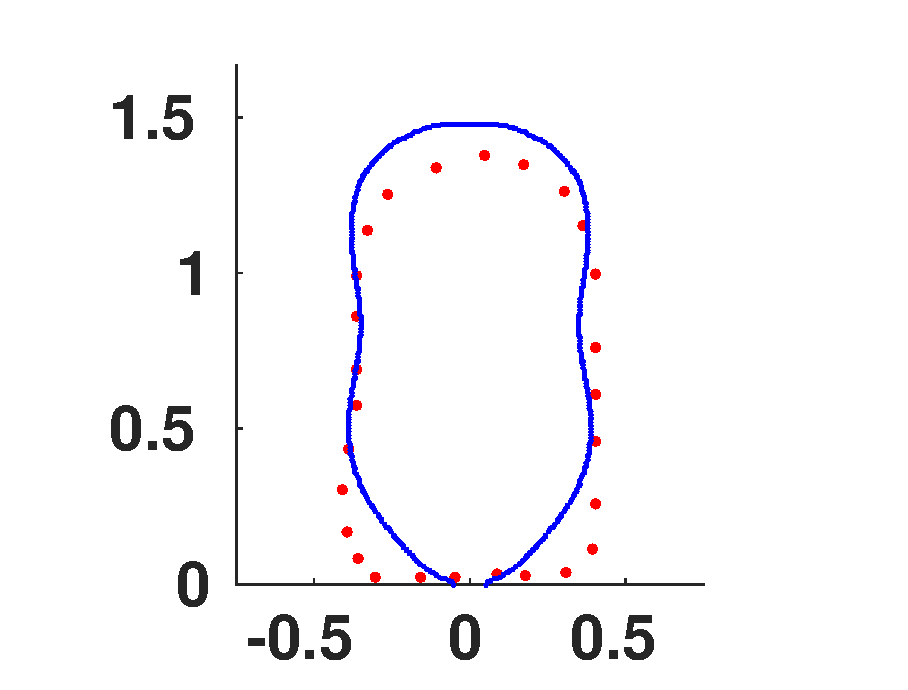
\includegraphics[width=0.3\textwidth]{wang-4.eps}
      }
    \subfloat[t = 19.0 ]{%
      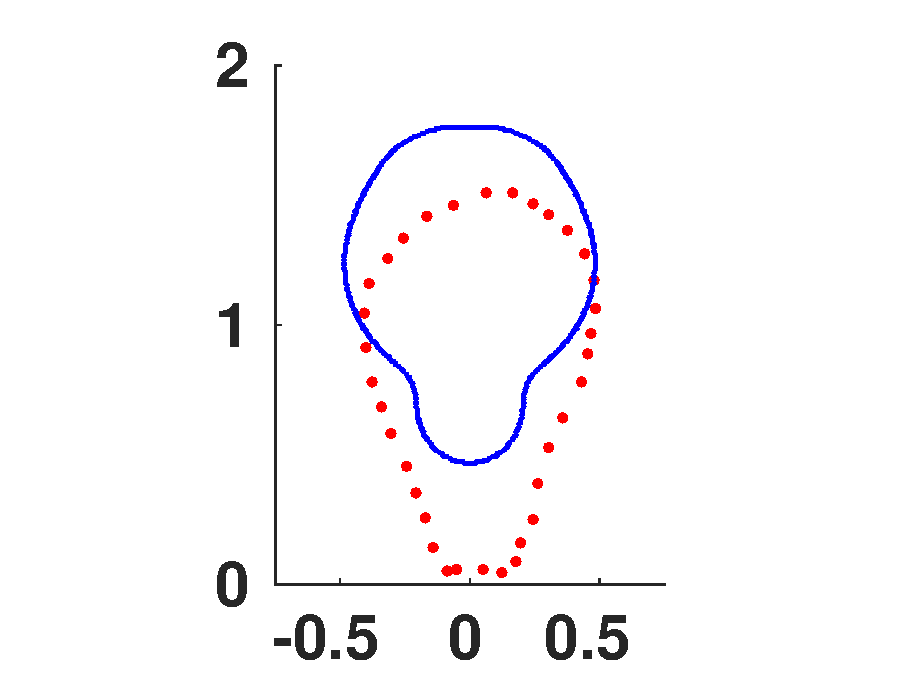
\includegraphics[width=0.3\textwidth]{wang-5.eps}
      }
       \subfloat[t = 19.5 ]{%
      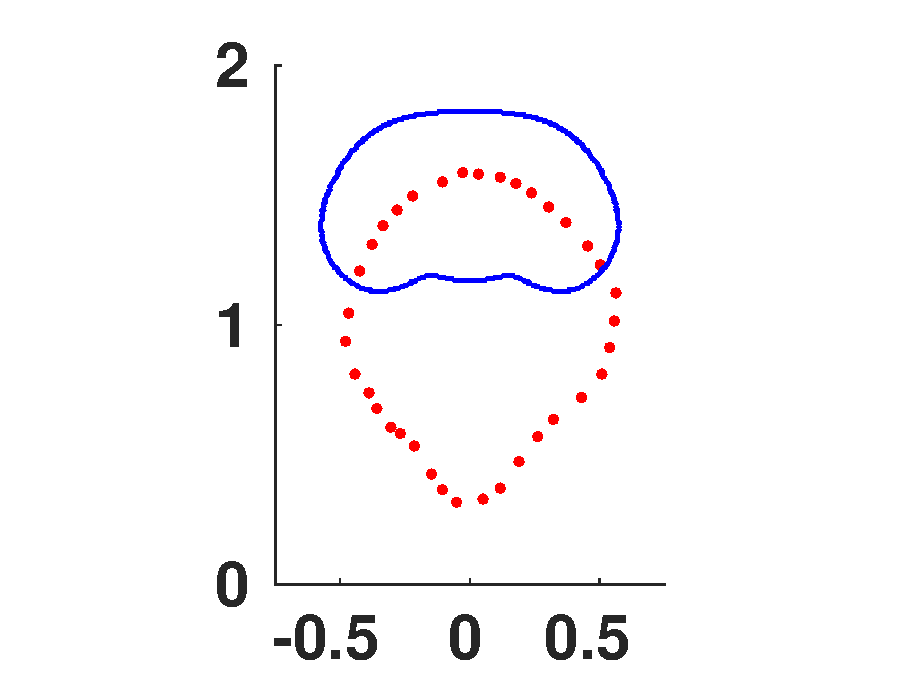
\includegraphics[width=0.3\textwidth]{wang-6.eps}
      }
    \caption{Interface Gerris simulation data(BLUE) with \cite{Wang2007} experimental data(RED)}
 \label{Fig:gs7}
 \end{figure}   
  \begin{figure}
 \centering
 \subfloat[t = 15.6 ]{%
      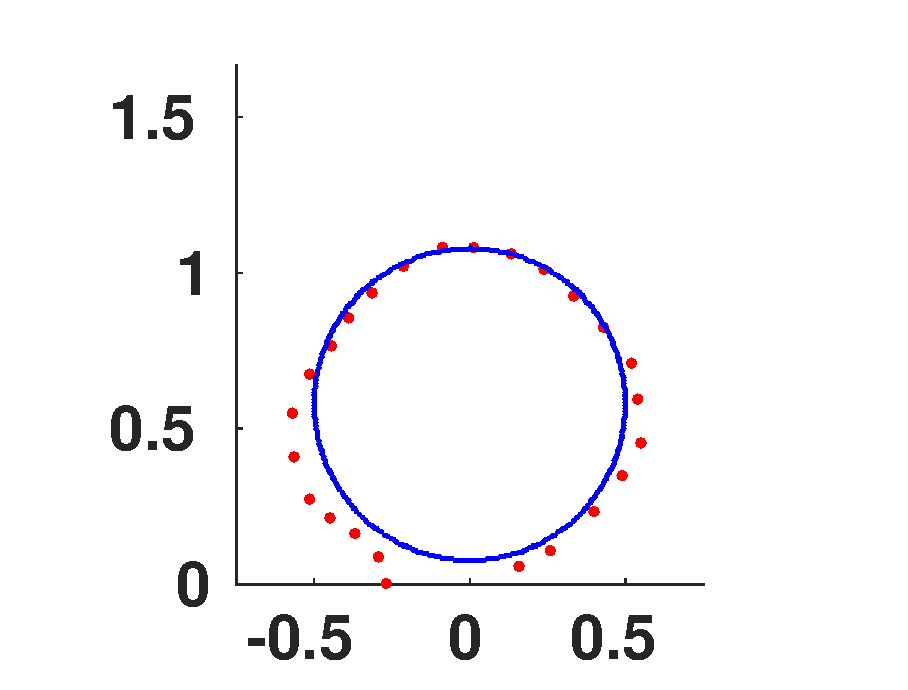
\includegraphics[width=0.3\textwidth]{wang-140-1.eps}
      }
  \subfloat[t = 16.6 ]{%
      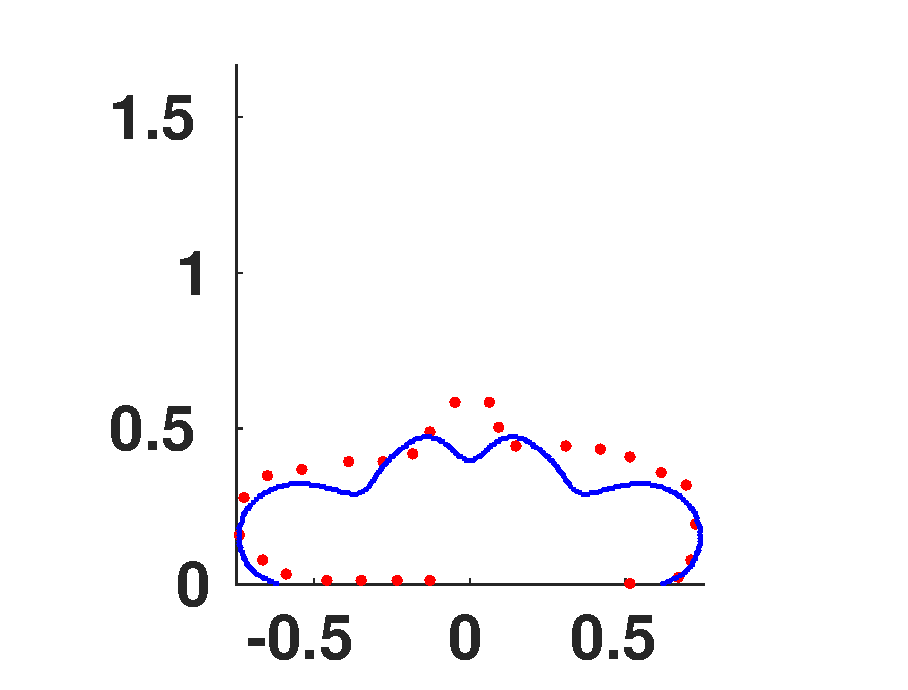
\includegraphics[width=0.3\textwidth]{wang-140-2.eps}
      } 
       \subfloat[t = 17.5 ]{%
      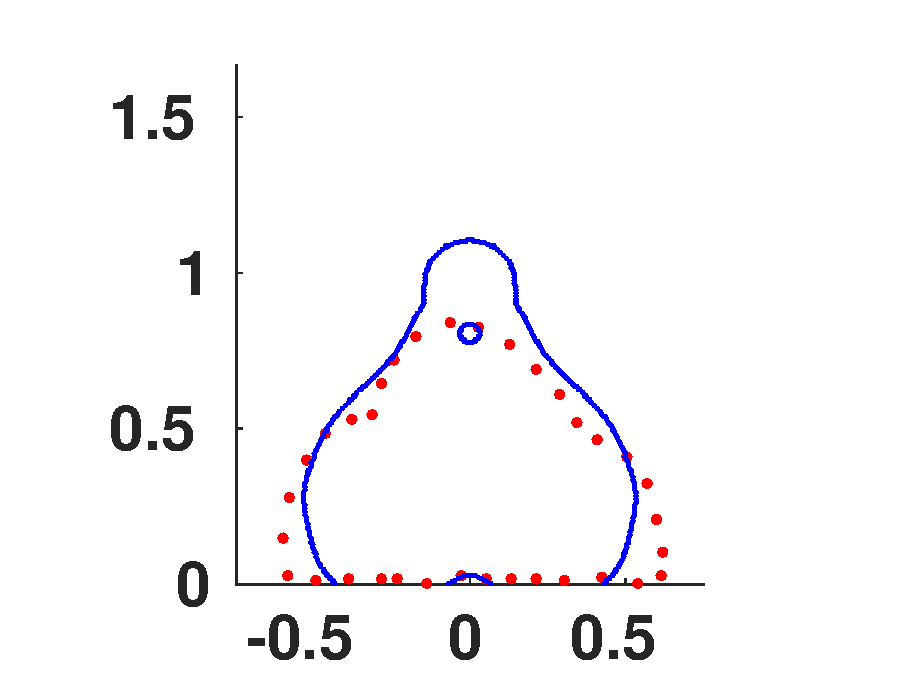
\includegraphics[width=0.3\textwidth]{wang-140-3.eps}
      }\\
       \subfloat[t = 20.4 ]{%
      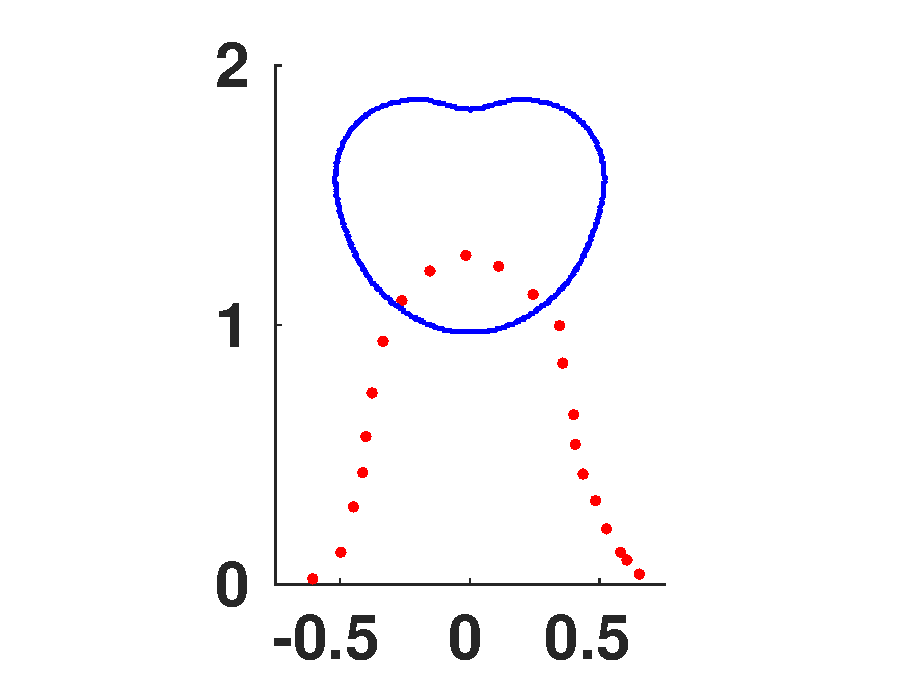
\includegraphics[width=0.3\textwidth]{wang-140-4.eps}
      }
    \subfloat[t = 21.9 ]{%
      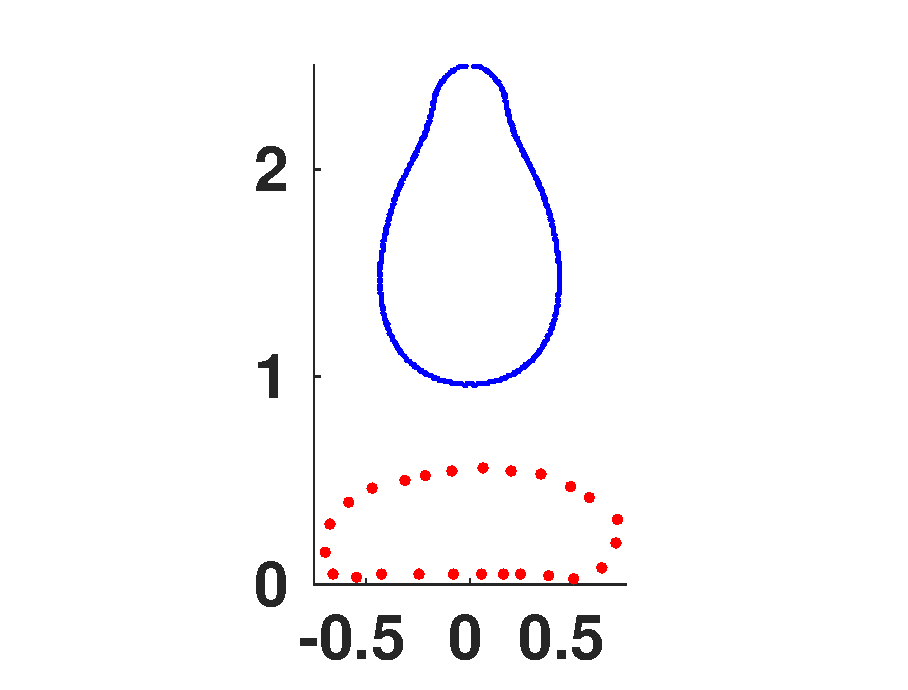
\includegraphics[width=0.3\textwidth]{wang-140-5.eps}
      }
       \subfloat[t = 24.6 ]{%
      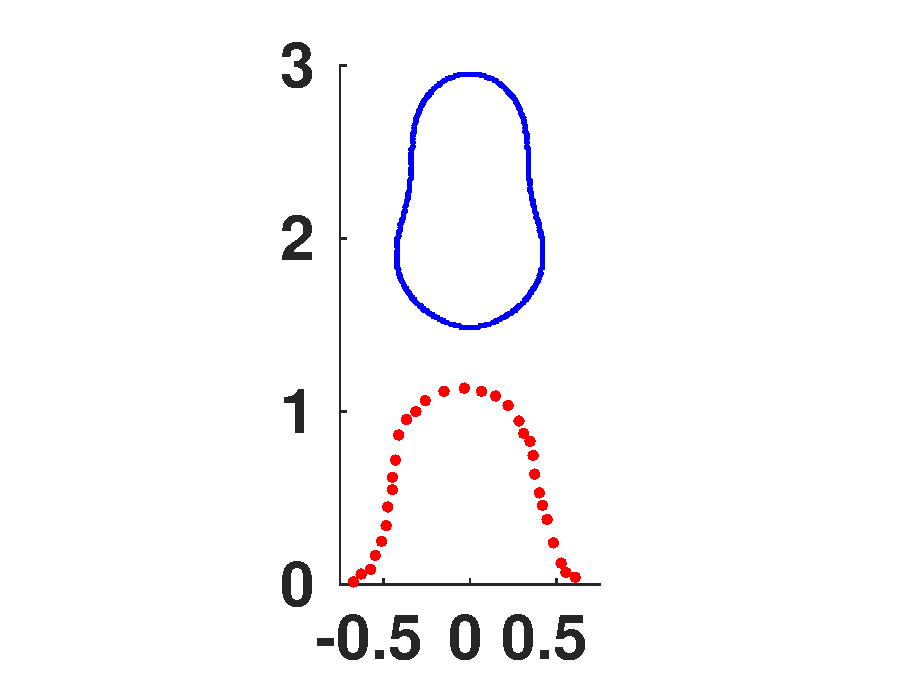
\includegraphics[width=0.3\textwidth]{wang-140-6.eps}
      }
    \caption{Interface Gerris simulation data(BLUE) with \cite{Wang2007} experimental data(RED)}
 \label{Fig:gs8}
 \end{figure}   